\documentclass[border=12pt]{standalone}
\usepackage{amssymb}
\usepackage{amsmath}
\usepackage{tikz}
\usetikzlibrary{arrows.meta, decorations.pathreplacing, calc, bending, positioning, shapes.geometric}

% Project palette (matches covering_diagram.tex)
\definecolor{cnavy}{HTML}{0E2747}
\definecolor{corange}{HTML}{E8573F}
\definecolor{cgreen}{HTML}{3B9B6D}
\definecolor{cslate}{HTML}{5B6680}
\definecolor{cmuted}{HTML}{9B9484}
\definecolor{ccream}{HTML}{FAFAF6}

\begin{document}
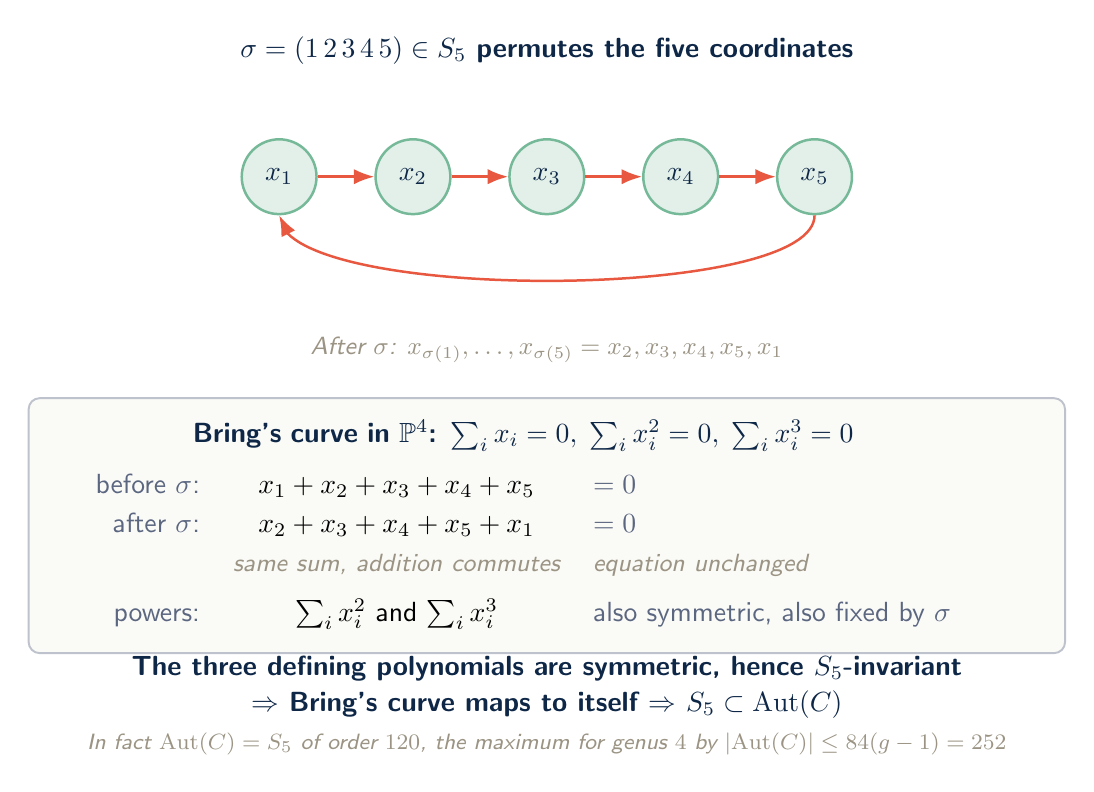
\begin{tikzpicture}[
  coord/.style={
    circle, draw=cgreen!70, fill=cgreen!15,
    line width=0.9pt, minimum size=0.95cm, inner sep=0pt
  },
  arrowG/.style={-{Latex[length=2.6mm]}, draw=corange, line width=0.9pt},
  eqbox/.style={
    rectangle, rounded corners=4pt, draw=cslate!40, fill=ccream,
    line width=0.7pt, inner sep=8pt
  },
  font=\sffamily
]

% ============================================================
% Top section: the action of sigma = (1 2 3 4 5) on the five coordinates.
\node[cnavy, font=\sffamily\bfseries] at (3.4, 6.20)
  {$\sigma = (1\,2\,3\,4\,5) \in S_5$ permutes the five coordinates};

% Five coordinate dots in a row
\foreach \i in {1,...,5} {
  \pgfmathsetmacro{\xpos}{(\i-1)*1.7}
  \node[coord] (x\i) at (\xpos, 4.6) {};
  \node[cnavy, font=\sffamily\bfseries] at (\xpos, 4.6) {$x_{\i}$};
}

% Adjacent arrows showing the cycle x_1 -> x_2 -> x_3 -> x_4 -> x_5
\foreach \i in {1,...,4} {
  \pgfmathtruncatemacro{\j}{\i+1}
  \draw[arrowG] (x\i.east) -- (x\j.west);
}
% Return arrow from x_5 back to x_1 (long curve below the row)
\draw[arrowG] (x5.south) .. controls (6.8, 3.0) and (0, 3.0) .. (x1.south);

% Result row underneath the cycle: x_{sigma(i)} = x_{i+1 mod 5}
\node[cmuted, font=\sffamily\itshape\small] at (3.4, 2.4)
  {After $\sigma$: $x_{\sigma(1)},\dots,x_{\sigma(5)} = x_2, x_3, x_4, x_5, x_1$};

% ============================================================
% Middle section: invariance of the three defining equations.
\node[eqbox, anchor=north, text width=12.6cm] (eqs) at (3.4, 1.8) {
  \begin{minipage}{12.0cm}
    \centering
    \textcolor{cnavy}{\textbf{Bring's curve in $\mathbb{P}^4$:
      $\sum_i x_i = 0,\;\sum_i x_i^{2} = 0,\;\sum_i x_i^{3} = 0$}}\\[6pt]

    \begin{tabular}{rcl}
      \textcolor{cslate}{before $\sigma$:} &
      $x_1 + x_2 + x_3 + x_4 + x_5$ & \textcolor{cslate}{$= 0$} \\[2pt]
      \textcolor{cslate}{after $\sigma$:}  &
      $x_2 + x_3 + x_4 + x_5 + x_1$ & \textcolor{cslate}{$= 0$} \\[2pt]
      & {\small\itshape\textcolor{cmuted}{same sum,
        addition commutes}} & {\small\itshape\textcolor{cmuted}{equation unchanged}} \\[6pt]

      \textcolor{cslate}{powers:} &
      $\sum_i x_i^{2}$ and $\sum_i x_i^{3}$ &
      \textcolor{cslate}{also symmetric, also fixed by $\sigma$}
    \end{tabular}
  \end{minipage}
};

% ============================================================
% Bottom: conclusion banner.
\node[cnavy, font=\sffamily\bfseries] at (3.4, -1.65)
  {The three defining polynomials are symmetric, hence $S_5$-invariant};
\node[cnavy, font=\sffamily\bfseries] at (3.4, -2.10)
  {$\Rightarrow$ Bring's curve maps to itself $\Rightarrow$ $S_5 \subset \mathrm{Aut}(C)$};

% Side note (italic, smaller) referencing the Hurwitz bound
\node[cmuted, font=\sffamily\itshape\footnotesize, align=center] at (3.4, -2.60)
  {In fact $\mathrm{Aut}(C) = S_5$ of order $120$, the maximum for genus $4$
   by $|\mathrm{Aut}(C)| \le 84(g-1) = 252$};

\end{tikzpicture}
\end{document}
